\begin{frame}
  \frametitle{Artificial Neural Networks}
  \begin{figure}
    \centering
    \resizebox{0.7\textwidth}{!}{\begin{neuralnetwork}[height=5]
  \tikzstyle{input neuron}=[neuron, draw, fill=white]
  \tikzstyle{hidden neuron}=[neuron, draw, fill=white]
  \tikzstyle{output neuron}=[neuron, draw, fill=white]
  \tikzstyle{link} = [->, shorten <=0pt, node distance=\nn@layerspacing, thin, draw=black];
  \inputlayer[count=4, bias=false, title=Input\\layer]
  \hiddenlayer[count=5, bias=false, title=Hidden\\layer] \linklayers
  \outputlayer[count=3, title=Output\\layer] \linklayers
\end{neuralnetwork}
}
    \caption{A common ANN-structure represented by a directed graph.}
  \end{figure}
\end{frame}

%% \begin{frame}
%%   \frametitle{Artificial Neural Networks}
%%   \begin{itemize}
%%     \item Class of machine learning algorithms
%%       \begin{itemize}
%%         \item Loosely inspired by biological nervous systems
%%       \end{itemize}
%%     \item Collection of artificial neurons that are connected with
%%       each other
%%       \begin{itemize}
%%         \item Enables them to exchange signals along their connections
%%         \item Can be represented by a directed graph
%%       \end{itemize}
%%     \item Usually arranged in layers
%%       \begin{itemize}
%%         \item \textit{Input Layer} collects input signals and passes
%%           them on
%%         \item \textit{Hidden Layers} apply transformations to incoming
%%           signals and pass the outcomes further into the network
%%         \item \textit{Output Layer} applies a final transformation
%%           representing the networks' result
%%       \end{itemize}
%%     \item Goal: Convert input into meaningful output by applying
%%       multiple transformations
%%   \end{itemize}
%% \end{frame}

\begin{frame}
  \frametitle{Modeling Artificial Neurons}
  \begin{figure}
    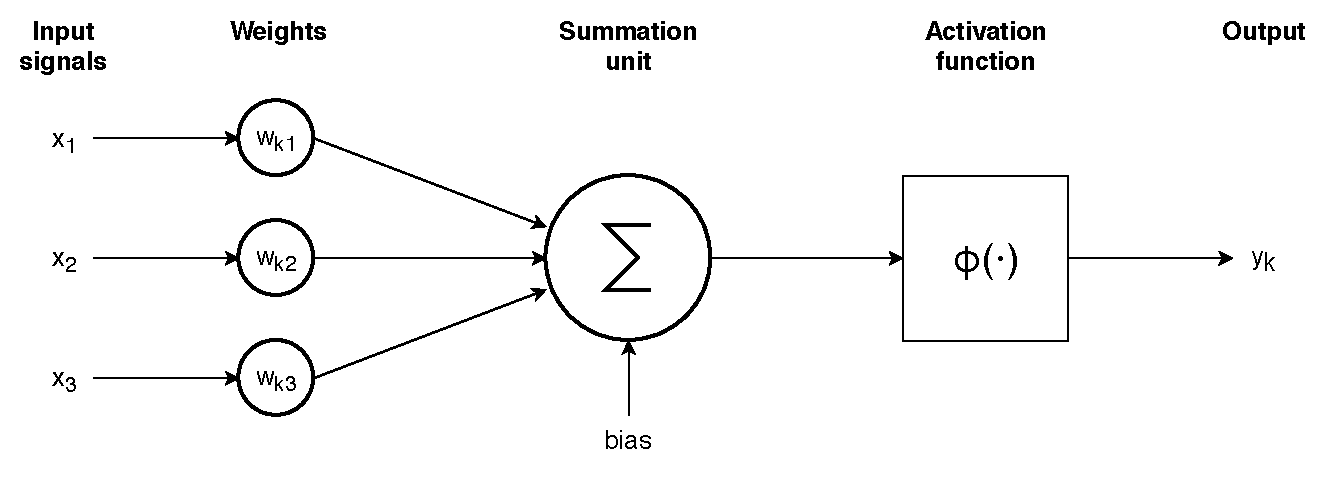
\includegraphics[width=.9\textwidth]{../figures/single_neuron}
    \caption{The components of a single artificial neuron \(k\).}
  \end{figure}
\end{frame}

%% \begin{frame}
%%   \frametitle{Components of the neural model}
%%   \begin{itemize}
%%    \item A set of weighted inputs
%%      \begin{itemize}
%%        \item Each input originating from neuron \(j\) and traveling
%%          into neuron \(k\) is first multiplied by a weight \(w_{kj}\)
%%      \end{itemize}
%%    \item A summation unit
%%      \begin{itemize}
%%        \item All the weighted inputs are summed and a constant value,
%%          the \textit{bias}, is added to yield the result \(z_k\)
%%      \end{itemize}
%%    \item An activation function
%%      \begin{itemize}
%%        \item Applies a non-linear transformation \(\phi(\cdot)\) to
%%          the output of the summation unit
%%        \item This result, called \(y_k\), is propagated further into
%%          the network alongside the connections
%%      \end{itemize}
%%   \end{itemize}
%% \end{frame}

\begin{frame}
  \frametitle{Activation Functions}
  \begin{itemize}
    \item Determine the ``activity''-level of a neuron based on the
      summed and weighted inputs
    \item Non-Linear
      \begin{itemize}
        \item Enables the network to model complex relations
        \item Multiple linear functions collapse into just a single
          linear function
      \end{itemize}
  \end{itemize}
\end{frame}

\begin{frame}
  \frametitle{Sigmoid Activation Function}
  \begin{equation}
    \phi(z) = \frac{1}{1 + e^{-\theta \cdot z}}
  \end{equation}
  \begin{itemize}
    \item Transforms an input into a range between 0 and 1
    \item \(\theta\) adjusts the sensitivity with respect to the input
    \item Reduces the impact of outliers
    \item Often used in the early days
      \begin{itemize}
        \item Biological inspiration, can also be interpreted as a ``firing-rate''
      \end{itemize}
  \end{itemize}
\end{frame}

\begin{frame}
  \frametitle{Sigmoid Activation Function}
  \begin{figure}
    \resizebox{.6\textwidth}{!}{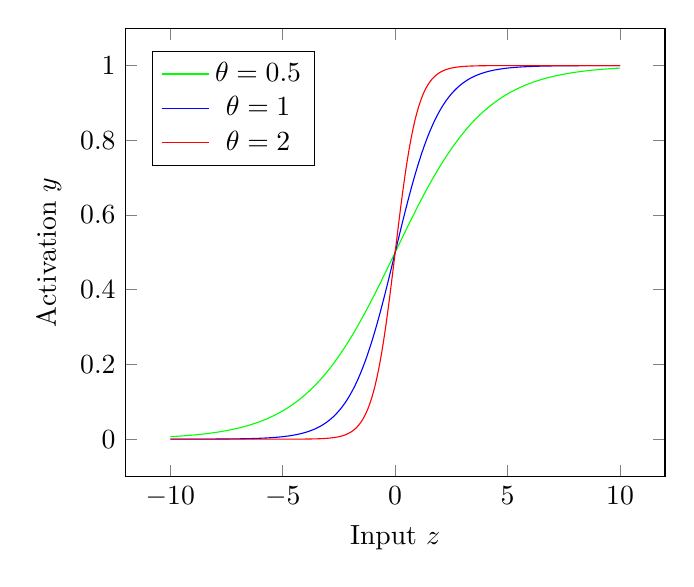
\begin{tikzpicture}
  \begin{axis}[
      xlabel={Input \(z\)},
      ylabel={Activation \(y\)},
      legend style={
        at={(0.05, 0.95)},
        anchor=north west
      }
    ]
    \addplot[green, domain=-10:10, samples=400]{1/(1+exp(-0.5*x))};
    \addplot[blue, domain=-10:10, samples=400]{1/(1+exp(-x))};
    \addplot[red, domain=-10:10, samples=400]{1/(1+exp(-2*x))};
    \legend{\(\theta = 0.5\), \(\theta = 1\), \(\theta = 2\)}
  \end{axis}
\end{tikzpicture}
}
    \caption{The sigmoid activation function plotted for different
      values of \(\theta\).}
  \end{figure}
\end{frame}

\begin{frame}
  \frametitle{Problems with the Sigmoid Activation Function}
  \begin{itemize}
    \item We sometimes want to keep big values
      \begin{itemize}
        \item Small values tend to fade out in deep networks (many
          hidden layers)
      \end{itemize}
    \item ``Saturates'' for very big or negative inputs, i.e. does
      not change much when the input changes
      \begin{itemize}
        \item This leads to training problems as we shall see later
      \end{itemize}
  \end{itemize}
\end{frame}

\begin{frame}
  \frametitle{ReLU Activation Function}
  \begin{equation}
    \phi(z) = \max(0, z)
  \end{equation}
  \begin{itemize}
    \item Remedies the problems of the sigmoid function
    \item Cuts away negative values \(\rightarrow\) sparsity among the
      neuron activations
      \begin{itemize}
        \item Promotes simpler representations
      \end{itemize}
    \item Actually more biologically inspired than the sigmoid
    \item Very easy to compute
  \end{itemize}
\end{frame}

\begin{frame}
  \frametitle{ReLU Activation Function}
  \begin{figure}
    \resizebox{.6\textwidth}{!}{\begin{tikzpicture}
  \begin{axis}[
      xlabel={Input \(z\)},
      ylabel={Activation \(y\)},
      legend style={
        at={(0.05, 0.95)},
        anchor=north west
      }
    ]
    \addplot[blue, domain=-10:10]{max(0, x)};
  \end{axis}
\end{tikzpicture}
}
    \caption{The ReLU activation function.}
  \end{figure}
\end{frame}

\begin{frame}
  \frametitle{Softmax Activation Function}
  \begin{equation}
    \phi(z_i) = \frac{e^{z_i}}{\sum_{j=1}^{n}{e^{z_j}}}
  \end{equation}
  \begin{itemize}
    \item Usually applied to the output neurons
    \item Outputs can be interpreted as probabilities
      \begin{itemize}
        \item Useful in classification, every possible class gets a
          probability
      \end{itemize}
    \item Using the exponential function before normalization
      amplifies bigger signals and attenuates weaker ones
      \begin{itemize}
        \item Helpful in training
      \end{itemize}
    \item Interpretation of the \(z_i\): Unnormalized
      log-probabilities
  \end{itemize}
\end{frame}

%% \begin{frame}
%%   \frametitle{The Role of the Bias Value}
%%   \begin{itemize}
%%     \item The bias is added as a constant to the sum of the weighted
%%       inputs in the summation unit
%%     \item Acts like a threshold that has to be overcome
%%       \begin{itemize}
%%         \item Negative bias: Positive weighted inputs needed for the
%%           neuron to become active
%%         \item Positive bias: Negative weighted inputs needed to stop
%%           the neuron from being active
%%       \end{itemize}
%%   \end{itemize}
%% \end{frame}

%% \begin{frame}
%%   \frametitle{The Role of the Bias Value}
%%   \begin{figure}
%%     \resizebox{.6\textwidth}{!}{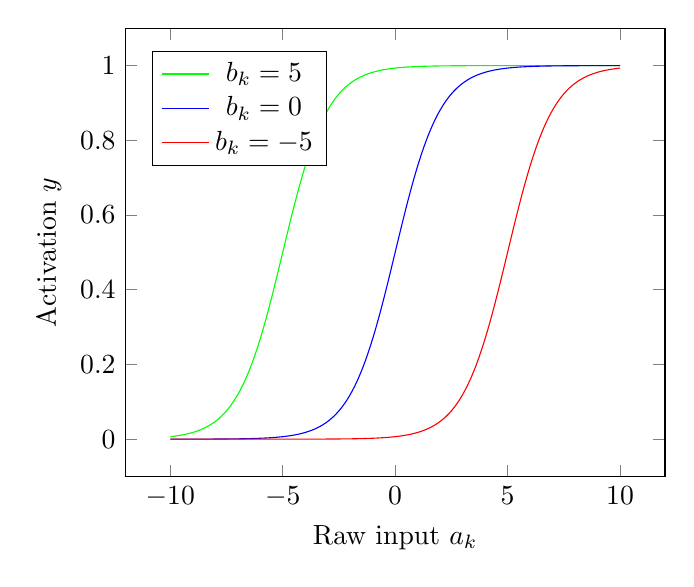
\begin{tikzpicture}
  \begin{axis}[
      xlabel={Raw input \(a_k\)},
      ylabel={Activation \(y\)},
      legend style={
        at={(0.05, 0.95)},
        anchor=north west
      }
    ]
    \addplot[green, domain=-10:10, samples=400]{1/(1+exp(-(x+5)))};
    \addplot[blue, domain=-10:10, samples=400]{1/(1+exp(-x))};
    \addplot[red, domain=-10:10, samples=400]{1/(1+exp(-(x-5)))};
    \legend{\(b_k = 5\), \(b_k = 0\), \(b_k = -5\)}
  \end{axis}
\end{tikzpicture}
}
%%     \caption{The sigmoid activation function plotted for different bias values.}
%%   \end{figure}
%% \end{frame}

\begin{frame}
  \frametitle{Neural Networks as Classifiers}
  \begin{itemize}
    \item We successfully established a mathematical model of neural
      networks
    \item How can we train them to perform classification tasks?
      \begin{itemize}
        \item Remember, we want to classify what kinds of faults are
          in a superlayer within the drift chamber
      \end{itemize}
    \item To do this, let's first take a look at classification in general
  \end{itemize}
\end{frame}

\begin{frame}
  \frametitle{Classification}
  \begin{itemize}
    \item The data consists of features as well as labels
    \item Goal: Predict the label by only looking at the features
    \item First step: Training
      \begin{itemize}
        \item The classification algorithm (classifier) is presented
          with many training examples
        \item For every new example, the classifier adjusts its
          parameters to improve its classification ability
        \item This is done to build a predictive model
      \end{itemize}
    \item Second step: Testing
      \begin{itemize}
        \item Some new testing examples are presented to the
          classifier that it did not see during training
        \item These examples are used to determine, if the classifier
          learned any useful concepts from the training data, i.e. to
          \textit{generalize}
      \end{itemize}
  \end{itemize}
\end{frame}

\begin{frame}
  \frametitle{Evaluating a Classifier}
  \begin{itemize}
    \item The results of the testing phase are entered into a
      \textit{confusion matrix:}
  \end{itemize}
  \begin{table}[h]
  \centering
  \renewcommand\theadfont{\bfseries}
  \begin{tabular}{|c|c|c|}
    \hline
    & \thead{Class Positive\\(Predicted)} & \thead{Class Negative\\(Predicted)} \\
    \hline
    \thead{Class Positive\\(Actual)} & True Positives (TP) & False
    Negatives (FN) \\
    \hline
    \thead{Class Negative\\(Actual)} & False Positives (FP) & True
    Negatives (TN) \\
    \hline
  \end{tabular}
  \end{table}
  \begin{itemize}
    \item This matrix is used to compute evaluation metrics like accuracy
  \end{itemize}
\end{frame}

%% \begin{frame}
%%   \frametitle{Evaluation Metrics}
%%   \begin{itemize}
%%     \item \textbf{Accuracy:}
%%       \begin{itemize}
%%         \item Percentage of testing examples that were classified correctly
%%       \end{itemize}
%%       \begin{equation}
%%         Accuracy = \frac{TP + TN}{TP + TN + FP + FN}
%%       \end{equation}
%%     \item \textbf{Precision:}
%%       \begin{itemize}
%%         \item Percentage of correctly classified examples among all
%%           examples classified as positive
%%       \end{itemize}
%%       \begin{equation}
%%         Precision = \frac{TP}{TP + FP}
%%       \end{equation}
%%   \end{itemize}
%% \end{frame}

%% \begin{frame}
%%   \frametitle{Evaluation Metrics}
%%   \begin{itemize}
%%     \item \textbf{Recall:}
%%       \begin{itemize}
%%         \item What percentage of positive examples was classified
%%           correctly?
%%       \end{itemize}
%%       \begin{equation}
%%         Recall = \frac{TP}{TP + FN}
%%       \end{equation}
%%     \item \textbf{F1 Score:}
%%       \begin{itemize}
%%         \item Harmonic mean of precision and recall
%%       \end{itemize}
%%       \begin{equation}
%%         \text{F1 Score} = \frac{2*Precision*Recall}{Precision+Recall}
%%       \end{equation}
%%   \end{itemize}
%% \end{frame}

\begin{frame}
  \frametitle{Training the Network}
  \begin{itemize}
    \item Which parameters can be adjusted during training?
      \begin{itemize}
        \item The weights and biases store the network's knowledge and
          need to be tuned to improve performance
        \item Other parameters like number of layers or activation
          function are set in advance (hyperparameters)
      \end{itemize}
    \item How to adjust the weights and biases?
      \begin{itemize}
        \item Measure the error on a batch of training examples
        \item Minimize the error by taking a step of \textit{gradient
          descent}
        \item Repeat this for a number of passes through the training
          data (one pass = one epoch)
      \end{itemize}
    \item After training, test the network on new examples
      \begin{itemize}
        \item Compute evaluation metrics
        \item Was it able to \textit{generalize}?
      \end{itemize}
  \end{itemize}
\end{frame}
